% Created 2020-04-22 mié 12:21
% Intended LaTeX compiler: pdflatex
\documentclass[presentation,aspectratio=169]{beamer}
\usepackage[utf8]{inputenc}
\usepackage[T1]{fontenc}
\usepackage{graphicx}
\usepackage{grffile}
\usepackage{longtable}
\usepackage{wrapfig}
\usepackage{rotating}
\usepackage[normalem]{ulem}
\usepackage{amsmath}
\usepackage{textcomp}
\usepackage{amssymb}
\usepackage{capt-of}
\usepackage{hyperref}
\usepackage{khpreamble}
\usetheme{default}
\author{Kjartan Halvorsen}
\date{\today}
\title{Feedback on reports for PI-control of a pneumatic tank}
\hypersetup{
 pdfauthor={Kjartan Halvorsen},
 pdftitle={Feedback on reports for PI-control of a pneumatic tank},
 pdfkeywords={},
 pdfsubject={},
 pdfcreator={Emacs 26.3 (Org mode 9.3.6)}, 
 pdflang={English}}
\begin{document}

\maketitle

\section{Feedback}
\label{sec:org5d43272}

\begin{frame}[label={sec:org0aee4a0}]{Estimating the parameter of the model}
The model is \[\underbrace{\frac{dp}{dt}}_{y} = a\underbrace{(u_v-5)\sqrt{p_s-p}}_{x}, \]
fit \(a\) in \(y=ax\).
\begin{center}
  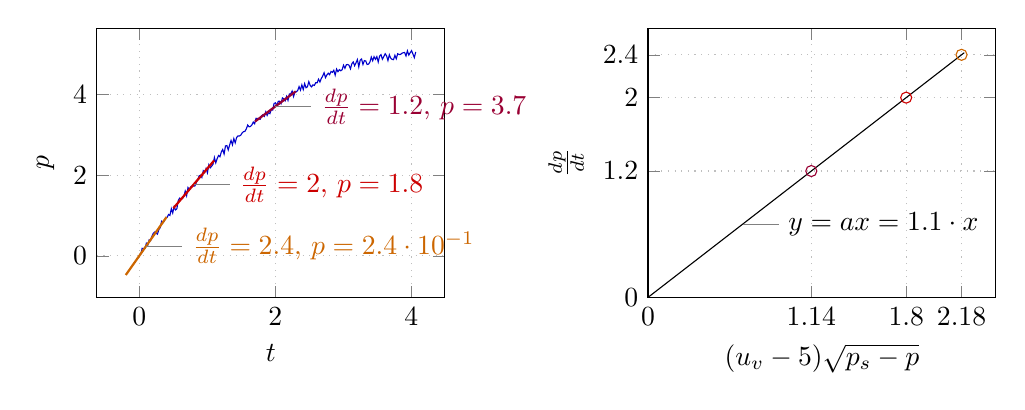
\begin{tikzpicture}
    \pgfmathsetmacro{\pps}{5}
    \pgfmathsetmacro{\aa}{1.1}
    \pgfmathsetmacro{\uv}{6}
    \pgfmathsetmacro{\AA}{\aa*(\uv-5)}
    \pgfmathsetmacro{\tmax}{2*sqrt(\pps)/\AA}
    \pgfmathsetmacro{\tone}{0.1}
    \pgfmathsetmacro{\pone}{\pps - pow(sqrt(\pps)-0.5*\AA*\tone,2)}
    \pgfmathsetmacro{\pdotone}{\AA*sqrt(\pps - \pone)}
    \pgfmathsetmacro{\ttwo}{0.8}
    \pgfmathsetmacro{\ptwo}{\pps - pow(sqrt(\pps)-0.5*\AA*\ttwo,2)}
    \pgfmathsetmacro{\pdottwo}{\AA*sqrt(\pps - \ptwo)}
    \pgfmathsetmacro{\tthree}{2}
    \pgfmathsetmacro{\pthree}{\pps - pow(sqrt(\pps)-0.5*\AA*\tthree,2)}
    \pgfmathsetmacro{\pdotthree}{\AA*sqrt(\pps - \pthree)}

    \pgfmathsetmacro{\xone}{(\uv-5)*sqrt(\pps-\pone)}
    \pgfmathsetmacro{\xtwo}{(\uv-5)*sqrt(\pps-\ptwo)}
    \pgfmathsetmacro{\xthree}{(\uv-5)*sqrt(\pps-\pthree)}

    \begin{axis}[
      clip=false,
      width = 6cm,
      height = 5cm,
      xlabel = {$t$},
      ylabel = {$p$},
      grid=both,
      major grid style = {dotted},
      ]
      \addplot[blue!80!black, no marks, domain=0:\tmax, samples=200,] {\pps - pow(sqrt(\pps)-0.5*\aa*x,2) + 0.1*rand};
      \addplot[orange!80!black, no marks, thick, domain=-0.3:0.3, samples=10] ({\tone+x}, {\pone + \pdotone*x}) node[coordinate, pos=0.5,pin=0:{$\frac{dp}{dt}=\pgfmathprintnumberto[precision=1]{\pdotone}{\myresult}\myresult$, $p=\pgfmathprintnumberto[precision=1]{\pone}{\myresult}\myresult$},] {}; 
      \addplot[red!80!black, no marks, thick, domain=-0.3:0.3, samples=10] ({\ttwo+x}, {\ptwo + \pdottwo*x}) node[coordinate, pos=0.5,pin=0:{$\frac{dp}{dt}=\pgfmathprintnumberto[precision=1]{\pdottwo}{\myresult}\myresult$, $p=\pgfmathprintnumberto[precision=1]{\ptwo}{\myresult}\myresult$},] {}; 
      \addplot[purple!80!black, no marks, thick, domain=-0.3:0.3, samples=10] ({\tthree+x}, {\pthree + \pdotthree*x}) node[coordinate, pos=0.5,pin=0:{$\frac{dp}{dt}=\pgfmathprintnumberto[precision=1]{\pdotthree}{\myresult}\myresult$, $p=\pgfmathprintnumberto[precision=1]{\pthree}{\myresult}\myresult$},] {}; 
    \end{axis}
    \begin{axis}[
      xshift=7cm,
      clip=false,
      width = 6cm,
      height = 5cm,
      xlabel = {$(u_v-5)\sqrt{p_s - p}$},
      ylabel = {$\frac{dp}{dt}$},
      yticklabel style={/pgf/number format/fixed,
                  /pgf/number format/precision=1},
      xtick = {0,\xthree, \xtwo, \xone},
      ytick = {0,\pdotthree,\pdottwo,\pdotone},
      grid=both,
      xmin=0,
      ymin=0,
      major grid style = {dotted},
      ]
      \addplot[orange!80!black, mark=o, ] coordinates {( \xone, \pdotone)};
      \addplot[red!80!black, mark=o, ] coordinates {( \xtwo, \pdottwo)};
      \addplot[purple!80!black, mark=o, ] coordinates {( \xthree, \pdotthree)};
      \addplot[black, no marks, domain=0:2.2, samples=20] { \aa*x } node[pos=0.3, coordinate, pin=0:{$y=ax=\aa \cdot x$},] {};
      \end{axis}
    
  \end{tikzpicture}
\end{center}
\end{frame}

\begin{frame}[label={sec:orgbfc8aab}]{The linearized model paramater \(b\) dependence on the operating pressure}
We obtained the following linearized models
\begin{align}
\frac{d}{dt}y(t) &= b_{in}u(t), \quad b_{in} = a\sqrt{p_s-p_0}, \quad \text{for air in}\\
\frac{d}{dt}y(t) &= b_{out}u(t), \quad b_{out} = a\sqrt{p_0}, \quad \text{for air out}
\end{align}

\begin{center}
  \begin{tikzpicture}
    \pgfmathsetmacro{\pps}{5}
    \pgfmathsetmacro{\aa}{1.1}
    \begin{axis}[
    clip=false,
    width=10cm,
    height=6cm,
    xlabel={$p_0$},
      ]
      \addplot[blue!80!black, no marks, domain=0:5, samples=100,] {\aa*sqrt(\pps-x)} node[pos=0.8,coordinate, pin=0:{$b_{in}$}] {};
      \addplot[orange!80!black, no marks, domain=0:5, samples=100,] {\aa*sqrt(x)} node[pos=0.2,coordinate, pin=0:{$b_{out}$}] {};
      \end{axis}
  \end{tikzpicture}
\end{center}
\end{frame}

\begin{frame}[label={sec:orgdd6eaa8}]{PI-controller design}
Using the controller \(F(s) = K\Big(1 + \frac{1}{sT_i}\Big) = K \frac{s T_i + 1}{sT_i}\)
 with \(T_i = 0.35\)
\begin{center}
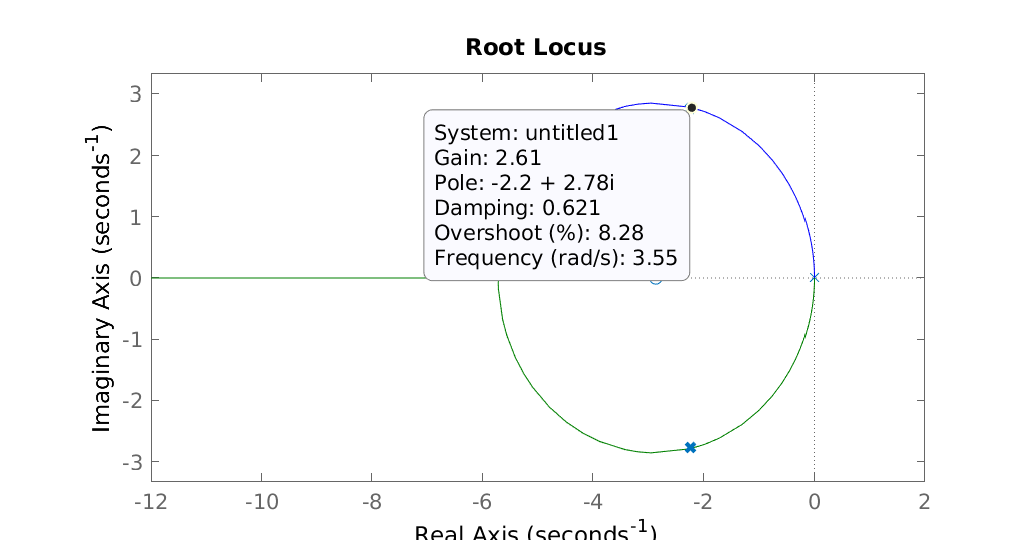
\includegraphics[width=0.7\linewidth]{../../figures/rlocus_PI_tank.pdf}
\end{center}
\end{frame}

\begin{frame}[label={sec:org242b71c}]{PI-controller design, contd}
The (linear) closed-loop system becomes
\[ G_c(s) = \frac{4.43s + 12.7}{s^2 + 4.43s + 12.7}\]

\begin{center}
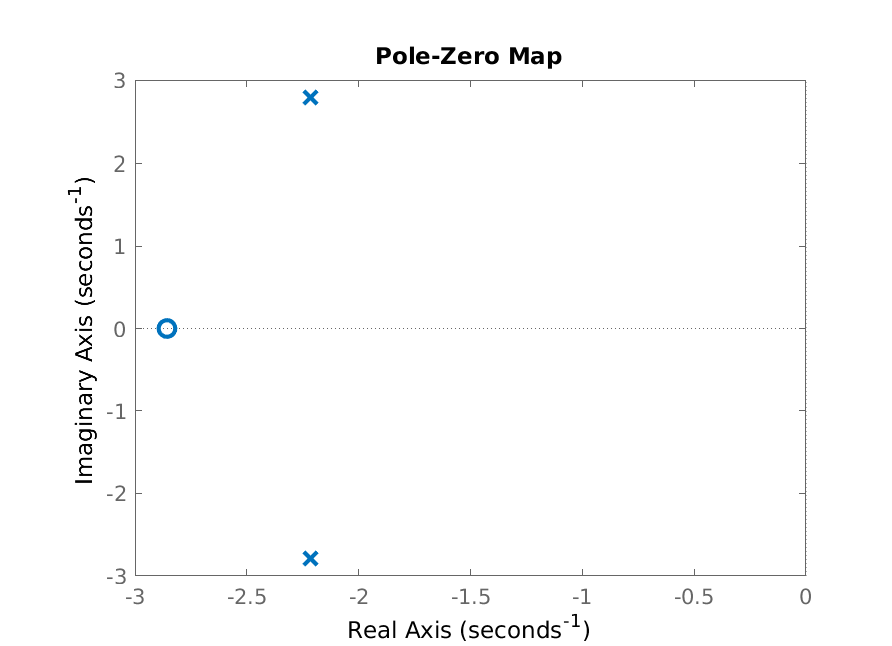
\includegraphics[width=0.6\linewidth]{../../figures/pzmap_PI_tank.pdf}
\end{center}
\end{frame}

\begin{frame}[label={sec:orgdca5f99}]{Simulations, P-controller}
\begin{center}
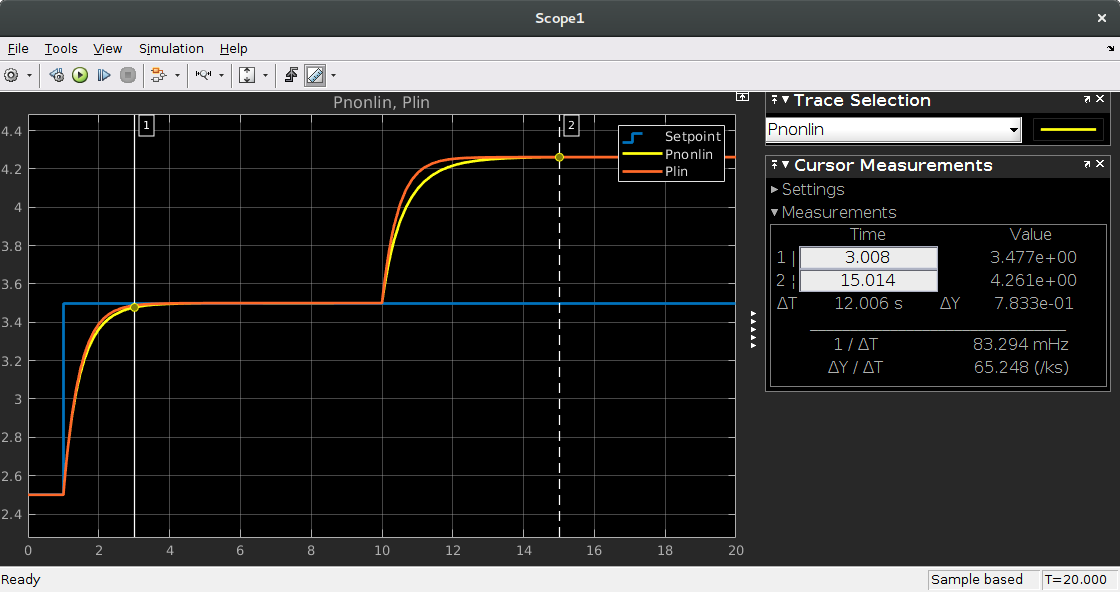
\includegraphics[width=1.0\linewidth]{../../figures/sim-P-control-tank.png}
\end{center}
\end{frame}
\begin{frame}[label={sec:org4949533}]{Simulations, PI-controller}
\begin{center}
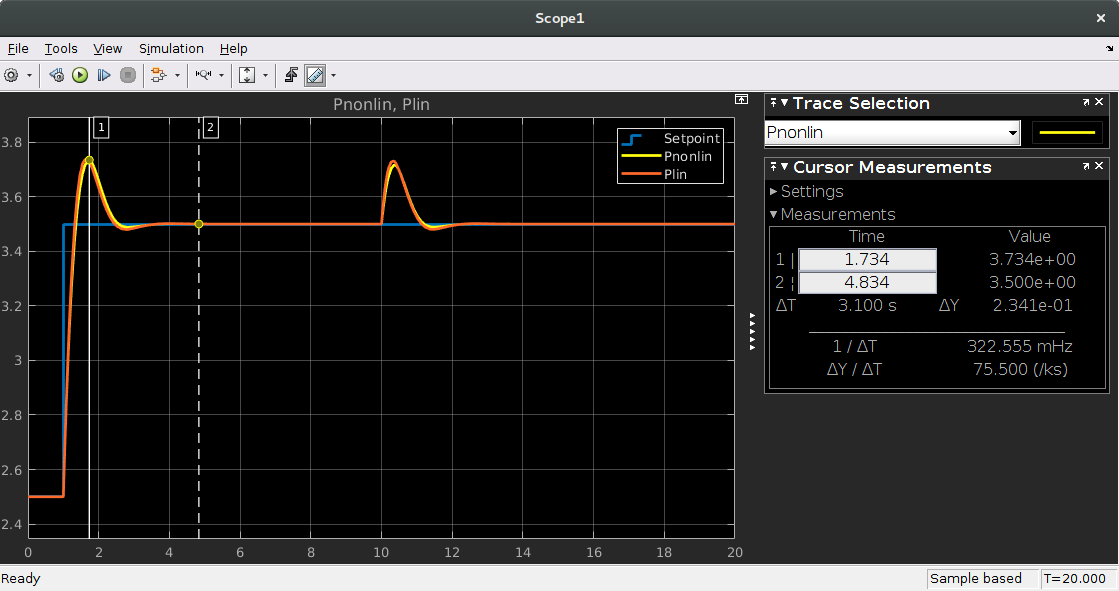
\includegraphics[width=1.0\linewidth]{../../figures/sim-PI-control-tank.png}
\end{center}
\end{frame}
\end{document}